\documentclass[tikz,border=12pt]{standalone}
\usepackage[T1]{fontenc}
\usepackage{mathpazo}
\usepackage{amsmath,amssymb}
\usetikzlibrary{arrows.meta, positioning, calc, fit, decorations.pathreplacing}

\definecolor{stblue}{HTML}{7B97AD}
\definecolor{rwgold}{HTML}{B8995E}
\definecolor{sage}{HTML}{7A9A7E}
\definecolor{dkbrown}{HTML}{3D3530}
\definecolor{wmgray}{HTML}{7B7067}
\definecolor{cream}{HTML}{F9F6F0}
\definecolor{border}{HTML}{D4C9B8}
\definecolor{terracotta}{HTML}{C47A6A}
\definecolor{lavender}{HTML}{907EA0}

\begin{document}
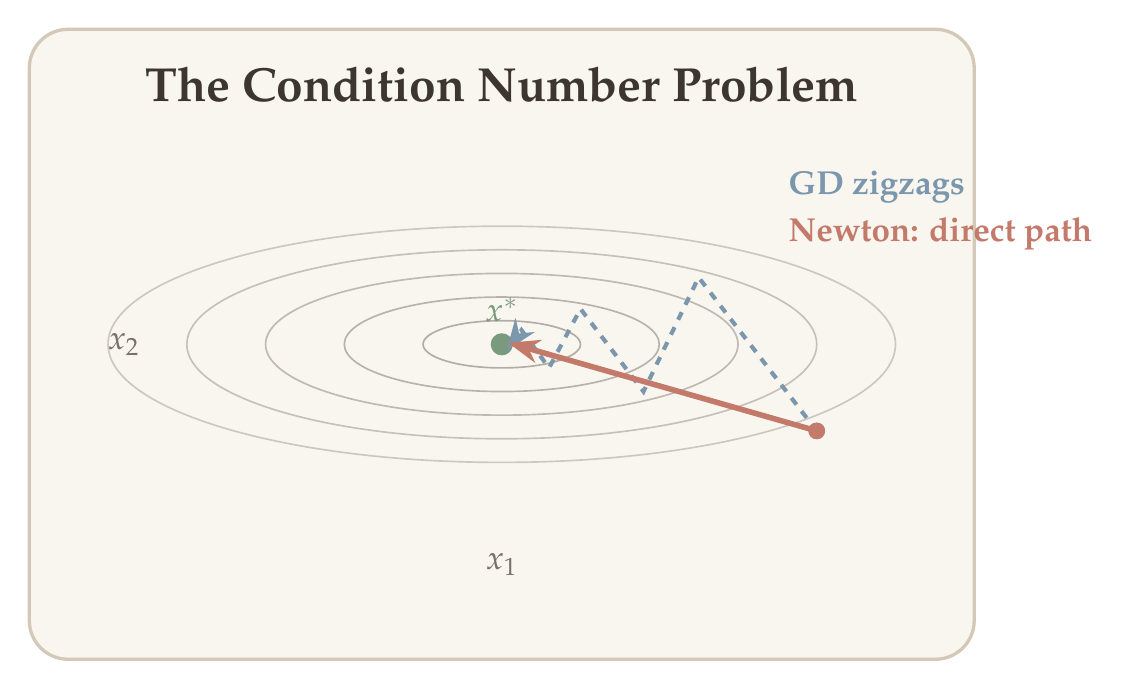
\begin{tikzpicture}[>={Stealth[length=4mm, width=3mm]}, line width=1.5pt]

% Background
\fill[cream, rounded corners=14pt] (-6.0,-4.0) rectangle (6.0,4.0);
\draw[border, line width=1.2pt, rounded corners=14pt] (-6.0,-4.0) rectangle (6.0,4.0);

% Title
\node[text=dkbrown, font=\LARGE\bfseries] at (0,3.3) {The Condition Number Problem};

% Contour ellipses (ill-conditioned: elongated horizontally)
\foreach \rx/\ry/\op in {1.0/0.3/0.55, 2.0/0.6/0.50, 3.0/0.9/0.45, 4.0/1.2/0.40, 5.0/1.5/0.35} {
  \draw[wmgray, line width=0.6pt, opacity=\op] (0,0) ellipse (\rx cm and \ry cm);
}

% Optimum star
\fill[sage] (0,0) circle (4pt);
\node[text=sage, font=\large\bfseries, above=4pt] at (0,0) {$x^*$};

% GD zigzag path
\draw[stblue, line width=1.5pt, dashed, ->]
  (4.0,-1.1) -- (2.5,0.85) -- (1.8,-0.6) -- (1.0,0.45)
  -- (0.6,-0.3) -- (0.25,0.18) -- (0.06,-0.08);
\fill[stblue] (4.0,-1.1) circle (3pt);

% Newton direct path
\draw[terracotta, line width=2pt, ->]
  (4.0,-1.1) -- (0.08,0.02);
\fill[terracotta] (4.0,-1.1) circle (3pt);

% Labels
\node[text=stblue, font=\large\bfseries, anchor=west] at (3.5,2.0) {GD zigzags};
\node[text=terracotta, font=\large\bfseries, anchor=west] at (3.5,1.4) {Newton: direct path};

% Axis labels
\node[text=wmgray, font=\large] at (0,-2.8) {$x_1$};
\node[text=wmgray, font=\large] at (-4.8,0) {$x_2$};

\end{tikzpicture}
\end{document}
